\begin{figure}[htbp]

\begin{center}
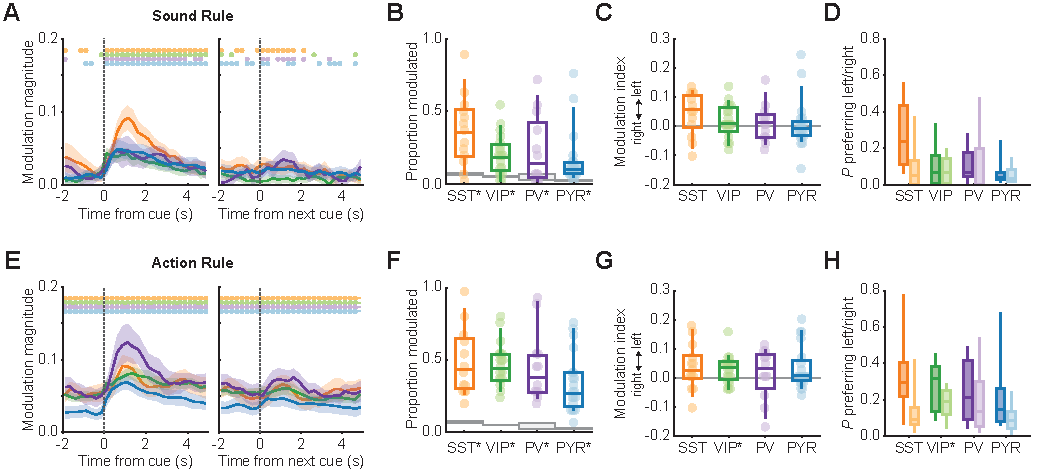
\includegraphics[width=\textwidth]{Figures/Chapter4/Fig6}
\end{center}

\caption[Choice-related modulation]
{Choice-related modulation. (A) Modulation magnitude $M$ with respect to the choice made in the current trial, plotted as a function of time relative to cue onset in the current trial (left) and the next trial (right). $M_{\mathit{choice}}(t)$ is presented as the difference from a null distribution obtained when the same analysis was conducted using shuffled choices. Line plots with shaded confidence intervals represent the $\mathit{mean} \pm \mathit{SEM}$ within SST (orange), VIP (green), PV (purple), and PYR populations (blue). Solid circles above indicate time bins where the corresponding cell type differed significantly from chance ($p<0.05$, Wilcoxon signed-rank test vs. shuffle). (B) The proportion of each cell population $P_{\mathit{choice}}$ that exhibited significant choice-related modulation in the current trial. (C) The mean modulation index $\bar{I}_{\mathit{choice}}$, calculated from the first 5 s of the current trial. (D) The proportion of each cell population exhibiting a significant preference for left ($P^+$) and right choices ($P^-)$, represented respectively in paired box plots to the left and right. (E--H) Same as A--C, for action blocks. For B--D and F--H, boxes indicate quartiles 1--3 and whiskers indicate the 9th and 91st percentiles of the empirical distribution. Values from individual sessions are represented in the beeswarm plots. Grey boxes represent quartiles 1 and 3 of the null distribution (visually indistinguishable from zero in C and G). Asterisks in B--C and F--G indicate significant differences from the null distribution for each cell type; in D and H, they indicate significant differences between $P^+$ and $P^-$ within each cell type; both were assessed at $\alpha = 0.05$, Wilcoxon signed-rank test. $N=$ 13 SST, 19 VIP, 12 PV, and 20 PYR populations.}

\label{fig:Fig6}
\end{figure}